\documentclass{article} % Tipo de documento
\usepackage[utf8]{inputenc} % Permite el uso de caracteres del Español
\usepackage[T1]{fontenc}
\usepackage{graphicx}
\usepackage{xcolor}
\usepackage{float}

% Carátula del Artículo
\title{La atmósfera terrestre}
\author{Adrián Zatarain Alvarado}
\date{23 de Enero, 2018}

% Comentario invisible

\begin{document}
\maketitle % Crea el título

\section{Introducción}

Como parte de la actividad de la clase. Se tiene que elaborar un escrito usando LATEX, principalmente para conocer su funcionamiento y usarlo en futuros proyectos.


La atmósfera terrestre es uno de los componentes más importantes que posee nuestro planeta. Es una capa de gases que rodea a la Tierra y tiene ciertas cualidades especiales. Protege la vida terrestre creando la suficiente presión para que el agua líquida pueda estar en la superficie, también absorbe la radiación ultravioleta provista por nuestra estrella, al mismo tiempo que hace cálida la temperatura reteniendo el calor, y, por supuesto, reduciendo las temperaturas extremas entre el día y la noche.

\begin{figure}[h!]
  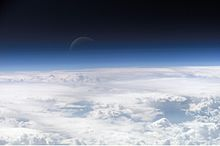
\includegraphics[0.50\width]{Top_of_Atmosphere.jpg}\centering
  \caption{La atmósfera terrestre}

  El halo azul característico es debido a que la luz azul se dispersa más.\centering

Imagen CC: Atmosphere of Earth (Wikipedia).}\centering


  \label{fig:La atmósfera terrestre}
\end{figure}




\section{Características de la atmósfera}

La atmósfera tiene distintas cualidades que la hacen destactar; que van desde su composición hasta sus propiedades más instrínsecas que ésta contiene. Dichas características la hacen especial. A continuación se describirán a detalle cada apartado.

\section{Composición}

La atmósfera contiene distintos gases, entre ellos se encuentran los tres más importantes; que son el nitrógeno, el oxígeno y el argón. El vapor de agua constituye aproximadamente el 0.25\% de la atmósfera por masa. En ésta, el vapor de agua varía alrededor de los 10 ppm por volumen en las partes más frías de la atmósfera a lo mucho en 5\% en volumen en masas de aire caliente y húmedo. La otra gama de gases son llamados gases traza, que son los gases invernaderos, los cuales lo conforman principalmente dióxido de carbono, metano, óxido nítrico y ozono.

El aire filtrado incluye combinaciones de muchos otros compuestos químicos. Muchas sustancias de origen natural pueden estar presentes en pequeñas cantidades estacionales y estacionalmente variables como aerosoles en una muestra de aire sin filtrar, que incluye polvo de minerales y composición orgánica, polen y esporas, rocío de mar y cenizas volcánicas.

Varios contaminantes industriales también pueden estar presentes en forma de gases o aerosoles, como cloro, compuestos de flúor y vapor de mercurio elemental. Los compuestos de azufre como el sulfuro de hidrógeno y el dióxido de azufre pueden derivarse de fuentes naturales o de la contaminación del aire industrial.

En la siguiente tabla se muestra los mayores constituyentes del aire




\begin{center}
    \begin{tabular}{| l | l | l | l |}
    \hline
    Nombre & Fórmula & V. en Pascales & En porcentaje \\ \hline
    Nitrógeno & N_2\ & 780 840 & 78.084. \\ \hline
    Oxígeno & O_2 & 209 460 & 20.946 \\ \hline
    Argón & Ar & 9 340 & 0.9340 \\ \hline
    Dióxido de carbono & CO_2 & 400 & 0.04 \\ \hline
    Neón & Ne & 18.18 & 0.001818 \\ \hline
    Helio & He & 5.24 & 0.000524 \\ \hline
    Metano & CH_4 & 1.79 & 0.000179 \\
    \hline
    \end{tabular}
\end{center}

\section{Estructura}

La atmósfera se compone de capas. Al elevarse, la prsión del aire y la densidad disminuyen. El comportamiento de la temperatura proporciona una medida útil para distinguir las capas atmosféricas.

De esta manera, la atmósfera de la Tierra se puede dividir en cuatro si se ignora la exosfera; la atmósfera tiene cuatro capas principales, que son la troposfera, la estratosfera, la mesósfera y la termósfera.



\begin{figure}{H}
  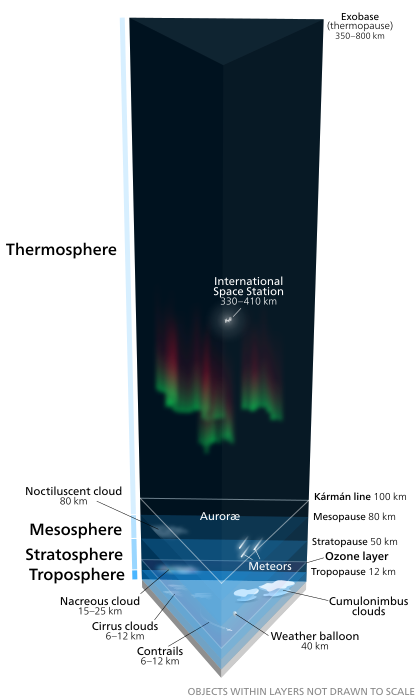
\includegraphics[height=10cm\width]{Capas.png}
  \caption{Las capas de la atmósfera terrestre}

  Se presentan las cuatro capas más icónicas de la Tierra\centering

Imagen CC: Atmosphere of Earth (Wikipedia).}\centering


  \label{fig:La atmósfera terrestre}
\end{figure}


A continuación se describe a detalle cada una:

\subsection{Exósfera}

La exosfera es la capa más externa de la atmósfera de la Tierra. tiene una extensión que va desde la exobase, que se encuentra en la parte superior de la termófera a una altitud de aproximadamente 700 km sobre el nivel del mar, a unos 10 000 km. Es en esa parte donde interactúa con el viento solar.

Se encuentra compuesta principalmente de densidades extremadamente bajas de hidrógeno, helio y varias moléculas más pesadas, incluyendo nitrógeno, oxígeno y dióxido de carbono. Los átomos y las moléculas están tan separados que pueden viajar cientos de kilómetros sin colisionar entre sí.

La exosfera se encuentra muy por encima de la Tierra para que sea posible cualquier fenómeno meteorológico. Sin embargo, la aurora boreal y la aurora austral a veces se encuentran en la parte inferior de la exosfera, donde se superponen a la termósfera. La exosfera contiene la mayoría de los satélites que orbitan alrededor de la Tierra.

\subsection{Termósfera}

Es la segunda capa más alta se extiende desde la mesopausia a una altitud de aproximadamente 80 km hasta la termopausa en un rango de altitud de 500-1000 km

La temperatura de la termósfera aumenta gradualmente con la altura. La actividad en la termósfera ocurre debido a la extremadamente baja densidad de sus moléculas. La temperatura de esta capa puede elevarse hasta 1500 grados centígrados, aunque las moléculas de gas están tan separadas que su temperatura en el sentido habitual no es muy significativa. El aire está tan rarificado que una molécula individual viaja un promedio de 1 kilómetro entre colisiones con otras moléculas.

Esta capa está completamente despejada y libre de vapor de agua. Sin embargo, fenómenos no hidrometeorológicos como la aurora boreal y la aurora austral se ven ocasionalmente en la termósfera. La Estación Espacial Internacional orbita en esta capa, entre 350 y 420 km.

\subsection{Mesósfera}

La mesósfera es la tercera capa más alta de la atmósfera de la Tierra, ocupando la región sobre la estratosfera y debajo de la termósfera. Se extiende desde la estrapaso a una altitud de aproximadamente 50 km a la mesopausia a 80-85 km sobre el nivel del mar.

Las temperaturas caen con el aumento de la altitud a la mesopausia que marca la parte superior de esta capa media de la atmósfera. Es el lugar más frío de la Tierra y tiene una temperatura promedio de alrededor de -85 grados centígrados.

La mesófera es también la capa donde la mayoría de los meteoros se queman al entrar en la atmósfera. Está demasiado elevado sobre la Tierra para que sea accesible para aviones y globos propulsados por aviones a reacción, y demasiado bajo para permitir naves espaciales orbitales. La mesósfera se accede principalmente por cohetes que suenan y aviones propulsados por cohetes.

\subsection{Estratósfera}

La estratosfera es la segunda capa más baja de la atmósfera de la Tierra. Se encuentra por encima de la troposfera y está separada de ella por la tropopausa. Esta capa se extiende desde la parte superior de la troposfera a aproximadamente 12 km de la superficie de la Tierra hasta la estratospausa a una altitud de aproximadamente 50 a 55 km.

La presión atmosférica en la parte superior de la estratosfera es aproximadamente 1/1000 de la presión al nivel del mar. Contiene la capa de ozono, que es la parte de la atmósfera de la Tierra que contiene concentraciones relativamente altas de ese gas. La estratosfera define una capa en la que las temperaturas aumentan con el aumento de la altitud. Este aumento de la temperatura es causado por la absorción de la radiación de la radiación ultravioleta del Sol por la capa de ozono, que restringe la turbulencia y la mezcla.

El perfil de temperatura estratosférico crea condiciones atmosféricas muy estables, por lo que la estratosfera carece de la turbulencia del aire que produce el clima y que prevalece en la troposfera.

\subsection{Tropósfera}

La troposfera es la capa más baja de la atmósfera de la Tierra. Se extiende desde la superficie de la Tierra hasta una altura promedio de aproximadamente 12 km, aunque esta altitud varía de unos 9 km en los polos a 17 km en el ecuador, con alguna variación debido al clima .

Casi todo el vapor de agua atmosférico o humedad se encuentra en la troposfera, por lo que es la capa donde tiene lugar la mayor parte del clima de la Tierra. La actividad de aviación más convencional tiene lugar en la troposfera, y es la única capa a la que se puede acceder mediante un avión propulsado por hélice.

\subsection{Otras capas}

\begin{itemize}

\item La capa de ozono está contenida dentro de la estratosfera. En esta capa, las concentraciones de ozono son aproximadamente de 2 a 8 partes por millón, que es mucho más alta que en la atmósfera más baja, pero aún muy pequeña en comparación con los componentes principales de la atmósfera. Se encuentra principalmente en la porción inferior de la estratosfera desde aproximadamente 15-35 km. \\

\item La ionosfera es una región de la atmósfera ionizada por la radiación solar. Es responsable de auroras. Durante el día, se extiende de 50 a 1,000 km e incluye la mesosfera, la termosfera y partes de la exosfera. Sin embargo, la ionización en la mesosfera cesa en gran medida durante la noche, por lo que las auroras normalmente se ven solo en la termosfera y la exosfera inferior. \\

\item La homósfera y la heterósfera se definen según si los gases atmosféricos están bien mezclados. La homósfera basada en la superficie incluye la troposfera, la estratosfera, la mesósfera y la parte más baja de la termosfera, donde la composición química de la atmósfera no depende del peso molecular porque los gases se mezclan por la turbulencia. Sobre esta altitud se encuentra la heterosfera, que incluye la exosfera y la mayor parte de la termosfera. Aquí, la composición química varía con la altitud. \\

\end{itemize}

\section{Propiedades físicas}


\subsection{Presión y espesor}

La presión atmosférica promedio a nivel del mar está definida por la Atmósfera Estándar Internacional como 101 325 pascales. Esto a veces se conoce como una unidad de atmósferas estándar. La masa atmosférica total es 5.1480 x 1018 kg, aproximadamente 2.5\% menos de lo que se deduciría de la presión media del nivel del mar y el área de la Tierra de 51007.2 megahectáreas, la presión del aire varía según la ubicación y el clima.


En resumen, la masa de la atmósfera de la Tierra se distribuye aproximadamente de la siguiente manera:

\begin{itemize}

\item 50\% está por debajo de 5.6 km.

\item 90\% está por debajo de 16 km.

\item 99.99997\% está por debajo de 100 km

\end{itemize}

\subsection{Temperatura y velocidad del sonido}

La división de la atmósfera en capas principalmente por referencia a la temperatura se discutió anteriormente. La temperatura disminuye con la altitud comenzando al nivel del mar, pero las variaciones en esta tendencia comienzan por encima de los 11 km, donde la temperatura se estabiliza a través de una gran distancia vertical a través del resto de la troposfera.

En la estratosfera, comenzando por encima de unos 20 km, la temperatura aumenta con la altura, debido al calentamiento dentro de la capa de ozono causado por la captura de radiación ultravioleta significativa del Sol por el dioxígeno y el gas ozono en esta región.


\begin{figure}{H}
  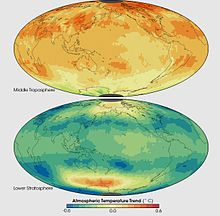
\includegraphics[height=5cm\width]{Atmospheric_Temperature_Trend.jpg}
  \caption{La temperatura del planeta}


Imagen CC: Atmosphere of Earth (Wikipedia).}\centering


  \label{fig:temperatura del planeta}
\end{figure}


\subsection{Densidad y masa}

La densidad del aire a nivel del mar es de aproximadamente 1.2 kg / m3 (1.2 g / L, 0.0012 g / cm3). La densidad no se mide directamente, pero se calcula a partir de mediciones de temperatura, presión y humedad utilizando la ecuación de estado para el aire. La densidad atmosférica disminuye a medida que aumenta la altitud. Esta variación se puede modelar aproximadamente utilizando la fórmula barométrica. Se usan modelos más sofisticados para predecir la desintegración orbital de los satélites. La masa promedio de la atmósfera es de aproximadamente 5 cuatrillones de la masa de la Tierra.


\section{Propiedades ópticas}

La radiación solar es la energía que recibe la Tierra del sol. La Tierra también emite radiación hacia el espacio, pero a longitudes de onda más largas que no podemos ver. Parte de la radiación entrante y emitida es absorbida o reflejada por la atmósfera. En mayo de 2017, se descubrió que los reflejos de luz de los cristales de hielo en la atmósfera reflejaban destellos de luz, que se veían centellear desde un satélite en órbita a un millón de millas de distancia.


\subsection{Dispersión}

Cuando la luz pasa a través de la atmósfera de la Tierra, los fotones interactúan con ella a través de la dispersión. Si la luz no interactúa con la atmósfera, se llama radiación directa y es lo que verá si mirara directamente al Sol. La radiación indirecta es luz que se ha dispersado en la atmósfera. Debido a que el Sol está cerca del horizonte, los rayos del Sol pasan a través de más atmósfera de lo normal para llegar a su ojo. Gran parte de la luz azul se ha dispersado, dejando la luz roja en una puesta de sol


\subsection{Absorción}

Diferentes moléculas absorben diferentes longitudes de onda de radiación. El agua absorbe muchas longitudes de onda por encima de 700 nm. Cuando una molécula absorbe un fotón, aumenta la energía de la molécula. Esto calienta la atmósfera, pero la atmósfera también se enfría al emitir radiación, como se explica a continuación.

Los espectros de absorción combinados de los gases en la atmósfera dejan "ventanas" de baja opacidad, permitiendo la transmisión de solo ciertas bandas de luz. La ventana óptica se extiende desde alrededor de 300 nm hasta el rango que los humanos pueden ver, el espectro visible, a aproximadamente 400-700 nm y continúa al infrarrojo a alrededor de 1100 nm. También hay ventanas de infrarrojos y de radio que transmiten algunas ondas infrarrojas y de radio a longitudes de onda más largas.


\subsection{Emisión}

La emisión es lo opuesto a la absorción, es cuando un objeto emite radiación. Los objetos tienden a emitir cantidades y longitudes de onda de radiación dependiendo de sus curvas de emisión de "cuerpo negro", por lo tanto, los objetos más calientes tienden a emitir más radiación, con longitudes de onda más cortas. Los objetos más fríos emiten menos radiación, con longitudes de onda más largas.

Debido a su temperatura, la atmósfera emite radiación infrarroja. El efecto invernadero está directamente relacionado con este efecto de absorción y emisión. Algunos gases en la atmósfera absorben y emiten radiación infrarroja, pero no interactúan con la luz solar en el espectro visible. Ejemplos comunes de estos son CO2 y H2O.

\subsection{Índice de refreacción}

El índice de refracción del aire es cercano, pero apenas superior a 1. Las variaciones sistemáticas en el índice de refracción pueden conducir a la flexión de los rayos de luz en recorridos ópticos largos. Un ejemplo es que, en algunas circunstancias, los observadores a bordo de barcos pueden ver otras embarcaciones justo sobre el horizonte porque la luz se refracta en la misma dirección que la curvatura de la superficie de la Tierra.

El índice de refracción del aire depende de la temperatura, dando lugar a efectos de refracción cuando el gradiente de temperatura es grande. Un ejemplo de tales efectos es el espejismo.


\section{Circulación}

La circulación atmosférica es el movimiento de aire a gran escala, y junto con la circulación oceánica es el medio por el cual la energía térmica se redistribuye en la superficie de la Tierra.

La circulación atmosférica de la Tierra varía de un año a otro, pero la estructura a gran escala de su circulación permanece bastante constante. Los sistemas meteorológicos a menor escala ocurren "aleatoriamente", y las predicciones meteorológicas a largo plazo de esas predicciones no pueden hacerse más allá de diez días en la práctica o un mes en teoría. El clima de la Tierra es consecuencia de su iluminación por el Sol y las leyes de la termodinámica. .


\subsection{Funciones de circulación latitudinal}

Los cinturones de viento que rodean al planeta están organizados en tres células en cada hemisferio: la célula de Hadley, la célula de Ferrel y la célula polar. Esas células existen en los hemisferios norte y sur. La mayor parte del movimiento atmosférico ocurre en la celda de Hadley. Los sistemas de alta presión que actúan sobre la superficie de la Tierra están equilibrados por los sistemas de baja presión en otros lugares. Como resultado, hay un equilibrio de fuerzas que actúa sobre la superficie de la Tierra


\subsection{Funciones de circulación longitudinal}

La circulación latitudinal es el resultado de la mayor radiación solar por unidad de área que cae sobre los trópicos. La intensidad solar disminuye a medida que aumenta la latitud, llegando prácticamente a cero en los polos. La circulación longitudinal, sin embargo, es el resultado de la capacidad calorífica del agua, su capacidad de absorción y su mezcla.

El agua absorbe más calor que la tierra, pero su temperatura no aumenta tanto como la tierra. Como resultado, las variaciones de temperatura en la tierra son mayores que en el agua.



\section{Bibliografía}

- Wikipedia. (2018, enero 28). Atmospheric of Earth. Obtenido de

https://en.wikipedia.org/wiki/Atmospheric\_circulation


\section{Apéndice}



1.- ¿Qué fue lo que más te llamó la atención de esta actividad?

         {\color{red}El cómo utilizar LATEX. Aprender cada comando, y cómo estructurar un texto. Me impresionó la cantidad de comandos existentes en LATEX y lo intuitivo que son}

2.- ¿Qué fue lo que se te hizo menos interesante?

        {\color{red}El tiempo que lleva el crear un documento, al igual que los contratiempos que lleva el redactar bien el código correspondiente.}

3.- ¿Qué cambios harías para mejorar esta actividad?

        {\color{red}Agregaría más fuentes de información y pondría un ejemplo más extenso con más instrucciones; como l¿para las imágenes. Escoger un mejor tema; que sea interesante y acorde a la carrera que se cursa.}

4.- ¿Cuál es tu primera impresión de uso de LATEX?

        {\color{red}Es bastante intuitivo, pero en veces frustante al tratar de poner código nuevo que no se conoce. Es un buen procesador de texto; lo hace todo muy elegante.}

5.- ¿El tiempo sugerido para esta actividad fue suficiente?
        {\color{red}Sí, fue suficiente. Es justo el necesario para realizarlo.}

6.- ¿Encontraste algún documento o recurso en línea útil que quisieras compartir con los demás?

        {\color{red}Sí. Indagando por internet encontré una página para hacer más extensa la síntesis sobre la atmósfera terrestre. Está adjunta en la bibliografía.}



\end{document}
